\documentclass[10pt,a4paper]{article}
\usepackage{algorithm}
\usepackage{algorithmicx}
\usepackage{algpseudocode}
\usepackage{amsfonts}
\usepackage{amsmath}
\usepackage{amssymb}
\usepackage{bbm}
\usepackage[a4paper, portrait, margin=1in]{geometry}
\usepackage{graphicx}
\usepackage{pdflscape}
\usepackage[utf8]{inputenc}
\author{Nathan Cunningham}
\title{MDI SMC: Progress Report}
\begin{document}
\maketitle

\section*{General algorithm}
\begin{algorithm}
\caption{Gibbs sampler}
 \begin{algorithmic}[1]
  \State Initialise $\Gamma$ matrix of prior allocation weights and $\Phi$ matrix of dataset concordance values
  \For{i = 1, \dots, number of iterations}
  \State Conditional on $\Gamma_{i-1}$ and $\Phi_{i-1}$ update the cluster labels, $c_{i}$, using alg. \ref{alg:pf}
  \State Conditional on $c_{i}$ update $\Gamma_i$ and $\Phi_i$
  \EndFor
\end{algorithmic}
\end{algorithm}


\begin{algorithm}
\caption{Particle filter to update cluster allocations}
\label{alg:pf}
 \begin{algorithmic}[1]
  \For{i = 1, \dots, n} \Comment{Loop over observations}
  \For{m = 1, \dots, M} \Comment{Loop over particles}
  \For{j = 1, \dots, d} \Comment{Loop over datasets}
  \State Sample $c^{(m)}_{i, j}$ \Comment{Propose a cluster for each datum}
  \State $q(c^{(m)}_{i,j} = k) \propto k^*(y_{i,j}|c_{i,j}^{(m)} = k) \gamma_{i, k, j}$ 
  \State $\xi^{(m)} =  \xi^{(m)} \times \gamma_{i, k, j}(1+\phi_{i})k^*(y_{i,k}|c_{i,j}^{(m)} = k)$ 
  \EndFor
  \EndFor
  \State Resample particles according to $\xi^{(m)}$
  \EndFor
  \State Update cluster labels using allocation in particle with largest $\xi^{(m)}$

\end{algorithmic}
\end{algorithm}

Where
\begin{equation}
\label{eq:likelihood}
k^*(y_{i, k}|c_{i, k}^{(m)} = k) = (\mathbf{y_{i, k}} - \mathbf{\mu_k}) \mathbf{\Sigma^{-1}} (\mathbf{y_{i, k}} - \mathbf{\mu_k})^\top
\end{equation}
\begin{equation}
\label{eq:phi}
\Phi \text{ is a measure of cluster label correspondence across datasets}
\end{equation}
\begin{equation}
\label{eq:gamma}
\gamma_{i, k, j} \text{ is a prior weight for assigning observation i, in dataset k to cluster j}
\end{equation}


\section{Algorithmic issues}
\begin{itemize}
\item Particle resampling step is currently disabled as it can crash the algorithm---possibly related to \texttt{NA} logweights being assigned.
\item Not currently taking advantage of parallel computing which means the algorithm is slower than it could be. It scales linearly with the number of particles.
\item As the MDI algorithm originally was not set up for multiple particles, a single particle is selected at the end of the particle filter (based on $\xi^{(m)}$) and that is fed into the next step of the Gibbs sampler. A possible solution would be to treat the particles as separate datasets, so all the particles are returned and the $\Gamma$ and $\Phi$ values are updated based on all of the particles.
\end{itemize}


\section{Multinomial data}
Extended the algorithm to work on multinomial data.

For each gene an observation is made on each of $Q$ features, each of which take a value $r$ from the set $\{1, \dots, R\}$. Denote the cluster-specific probability of getting value $r$ for feature $q$ by $\theta_{rq}^{(m)}$, such that $\Sigma_{r = 1}^{R} \theta_{rq}^{(m)} = 1$ for each particle, m. Adopt a $Dirichlet\{\beta_{1q}^{(m)}, \dots, \beta_{Rq}^{(m)}\}$ prior for $\theta_{1q}^{(m)}, \dots, \theta_{Rq}^{(m)}$. The Dirichlet prior hyperparameter, $\beta_{rq}^{(m)}$ is taken as $0.5$. Denote the resulting prior probabilities as $b_{rq}^{(m)}$

Assuming independence between features, the probability of assigning the $i^{th}$ observation to a cluster, j, in particle m is calculated as:

\begin{equation}
p(c_{i}^{(m)} = j| x_{1:i}^{(m)}, c_{1:(n - 1)}^{(m)},b_{1q}^{(m)}, \dots, b_{Rq}^{(m)}, a^{(m)} ) = 
\prod_{q = 1}^{Q} 
\frac{(n_{j, x_i}^{(m)} \times a^{(m)}) + (b_{rq}^{(m)} \times (1 - a^{(m)}))}
{(n_{j, \cdot}^{(m)} \times a^{(m)}) + (1 \times (1 - a^{(m)}))}
\end{equation}

Where $n_{j, x_i}^{(m)}$ is the number of observations in cluster $j$ with the same value as $x_i^{(m)}$,  $n_{j, \cdot}^{(m)}$ is the total number of observations in cluster $j$ and $a^{(m)}$ is a particle-specific centring measure. This is a weighted average of the empirical probability  of the value of $x_{i}$ in the cluster j, and the prior probability.

Output of the algorithm clustering multinomial and gaussian data is presented in Figures \ref{fig:multinom1} and \ref{fig:multinom2}.


\section{Markov chain diagnostics}
Convergence of the markov chain can be examined by viewing plots of the allocation agreement. Figure \ref{fig:agreement} shows the pairwise agreement of genes in clusters (``fusion''). Although these are relatively stable there appears to be some evidence of an upward trend, so it may be that the algorithm has not yet converged. The algorithm was run for $1000$ iterations.

Figure \ref{fig:agreement_hist} shows the distribution of pairwise allocation agreements. The x axis indicates the number of fused genes across the two datasets, while the height represents the frequency this occurs in the Markov chain. The number of genes fused appears to be uniformly distributed, when it should be hoped that in most cases a large number of genes are fused.






\begin{landscape}
\begin{figure}[htbp]
\label{fig:multinom1}
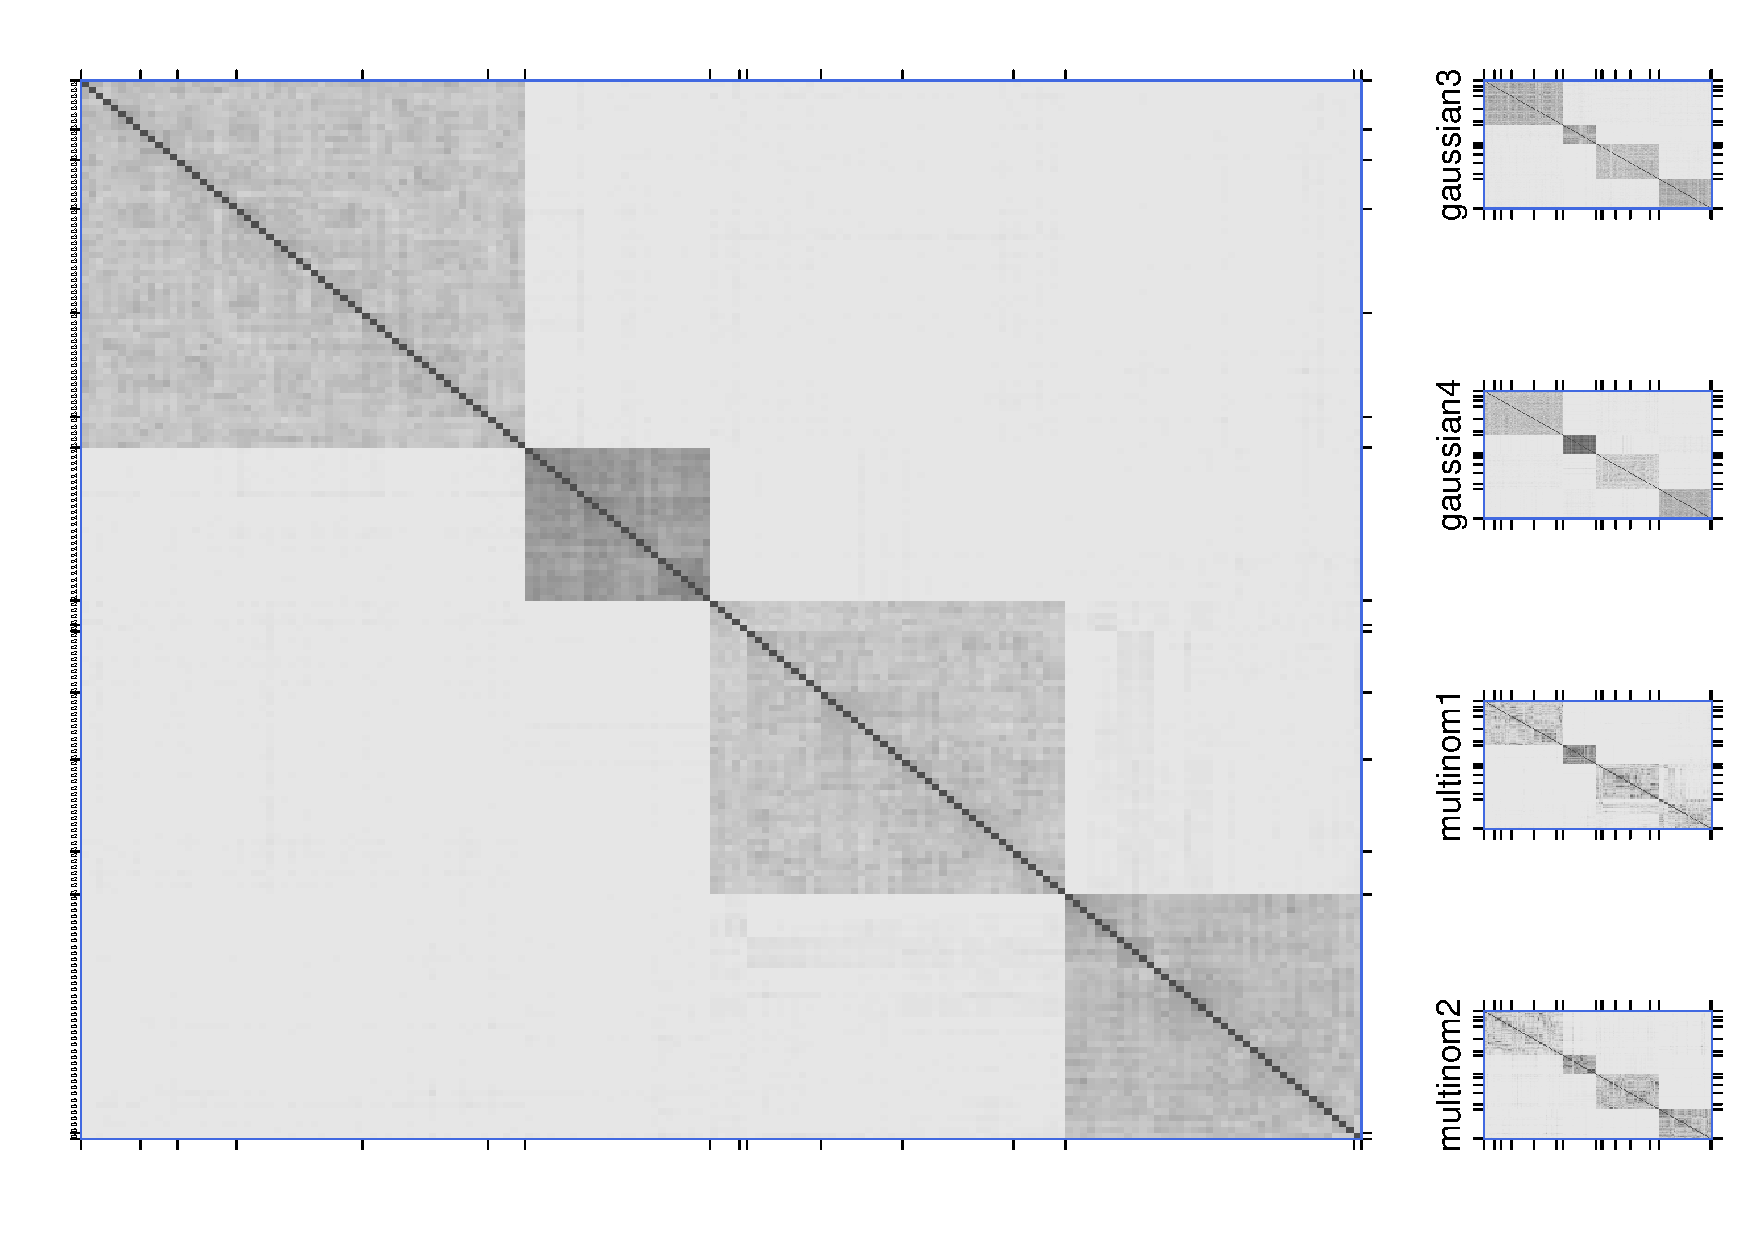
\includegraphics[width = 0.95\linewidth]{Plots/multinom_consensus.pdf}
\caption{Running MDI using four datasets: two gaussian and two multinomial, with a shared clustering order. The algorithm is attempting to partition the data into 15 clusters, but appears to be recovering the four true clusters.}
\end{figure}
\newpage
\begin{figure}[htbp]
\label{fig:multinom2}
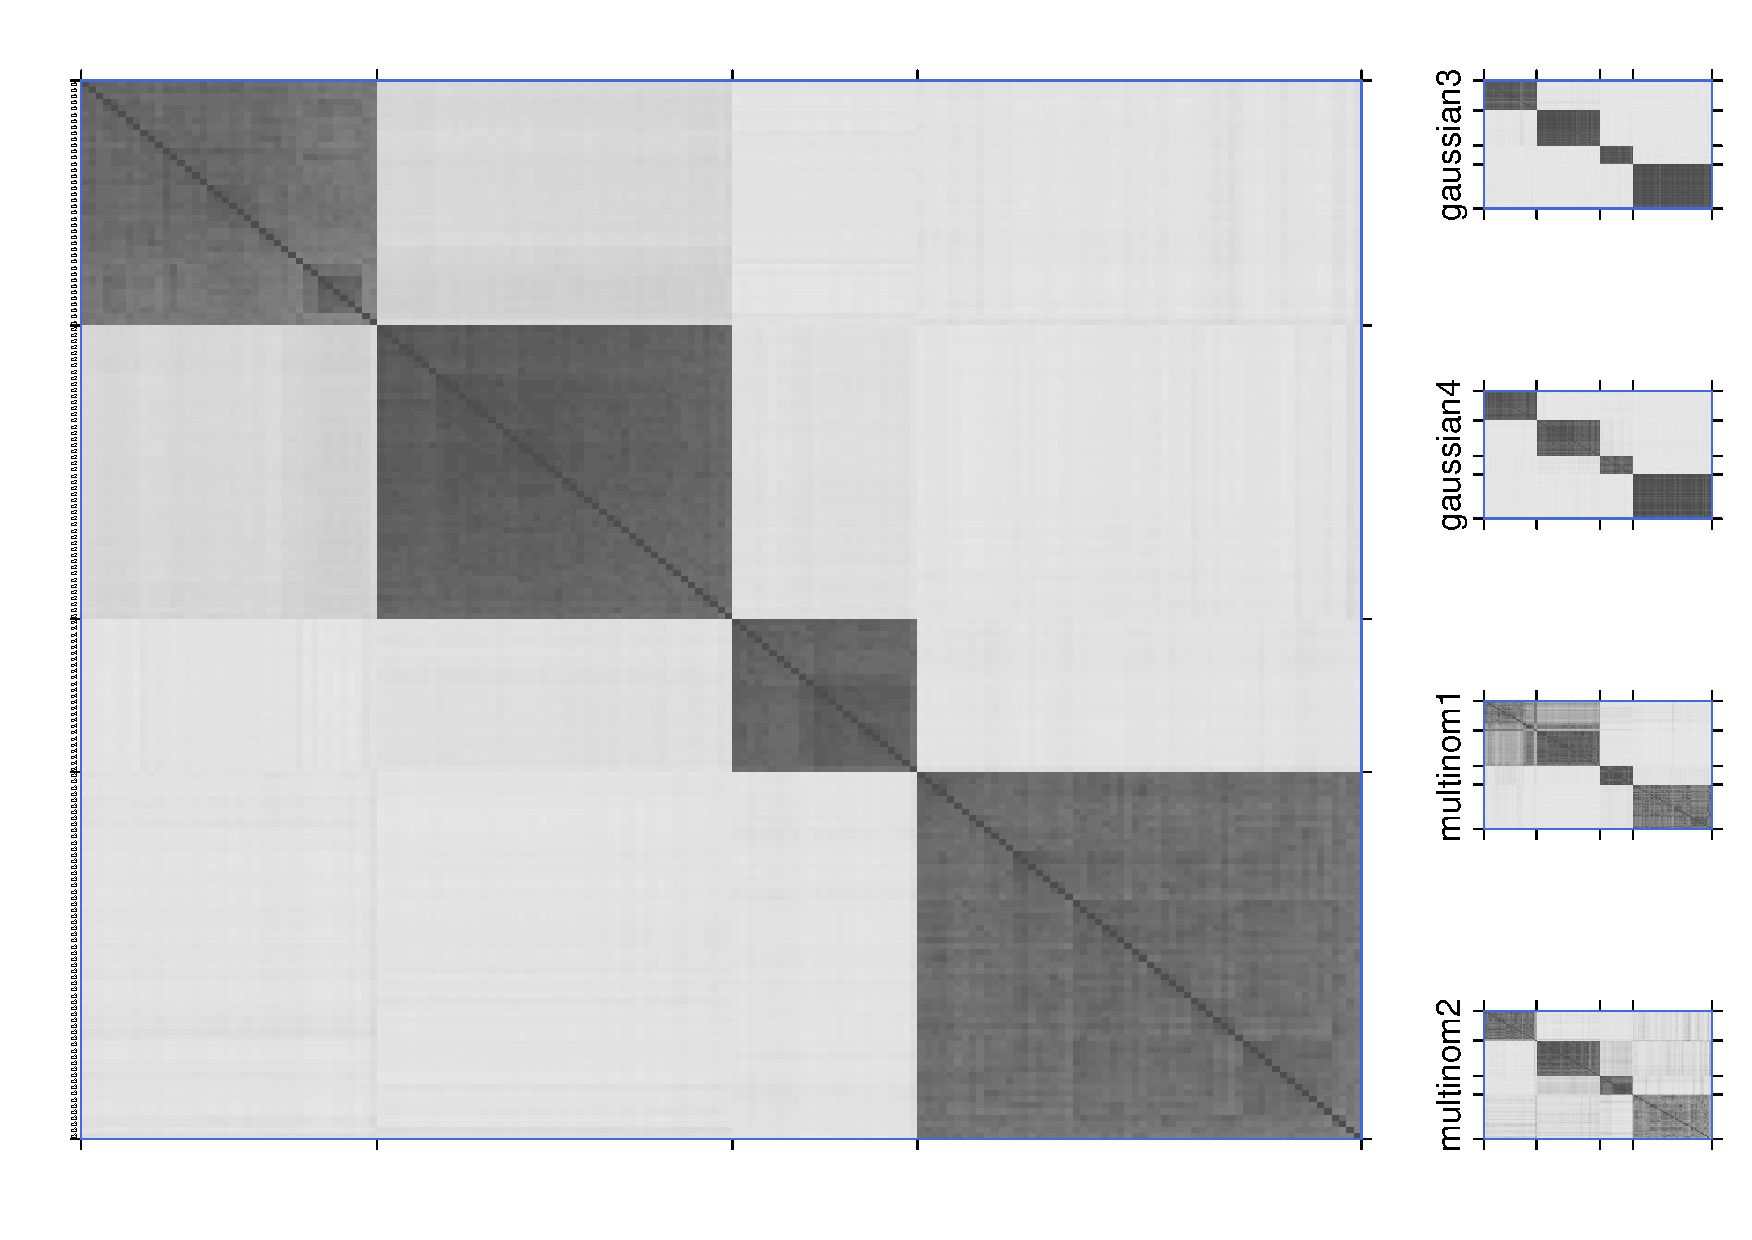
\includegraphics[width = 0.95\linewidth]{Plots/multinom_consensus_4.pdf}
\caption{Running MDI using four datasets: two gaussian and two multinomial, with a shared clustering order. The algorithm is attempting to partition the data into four clusters and is recovering the true clustering.}
\end{figure}

\begin{figure}[htbp]
\label{fig:agreement}
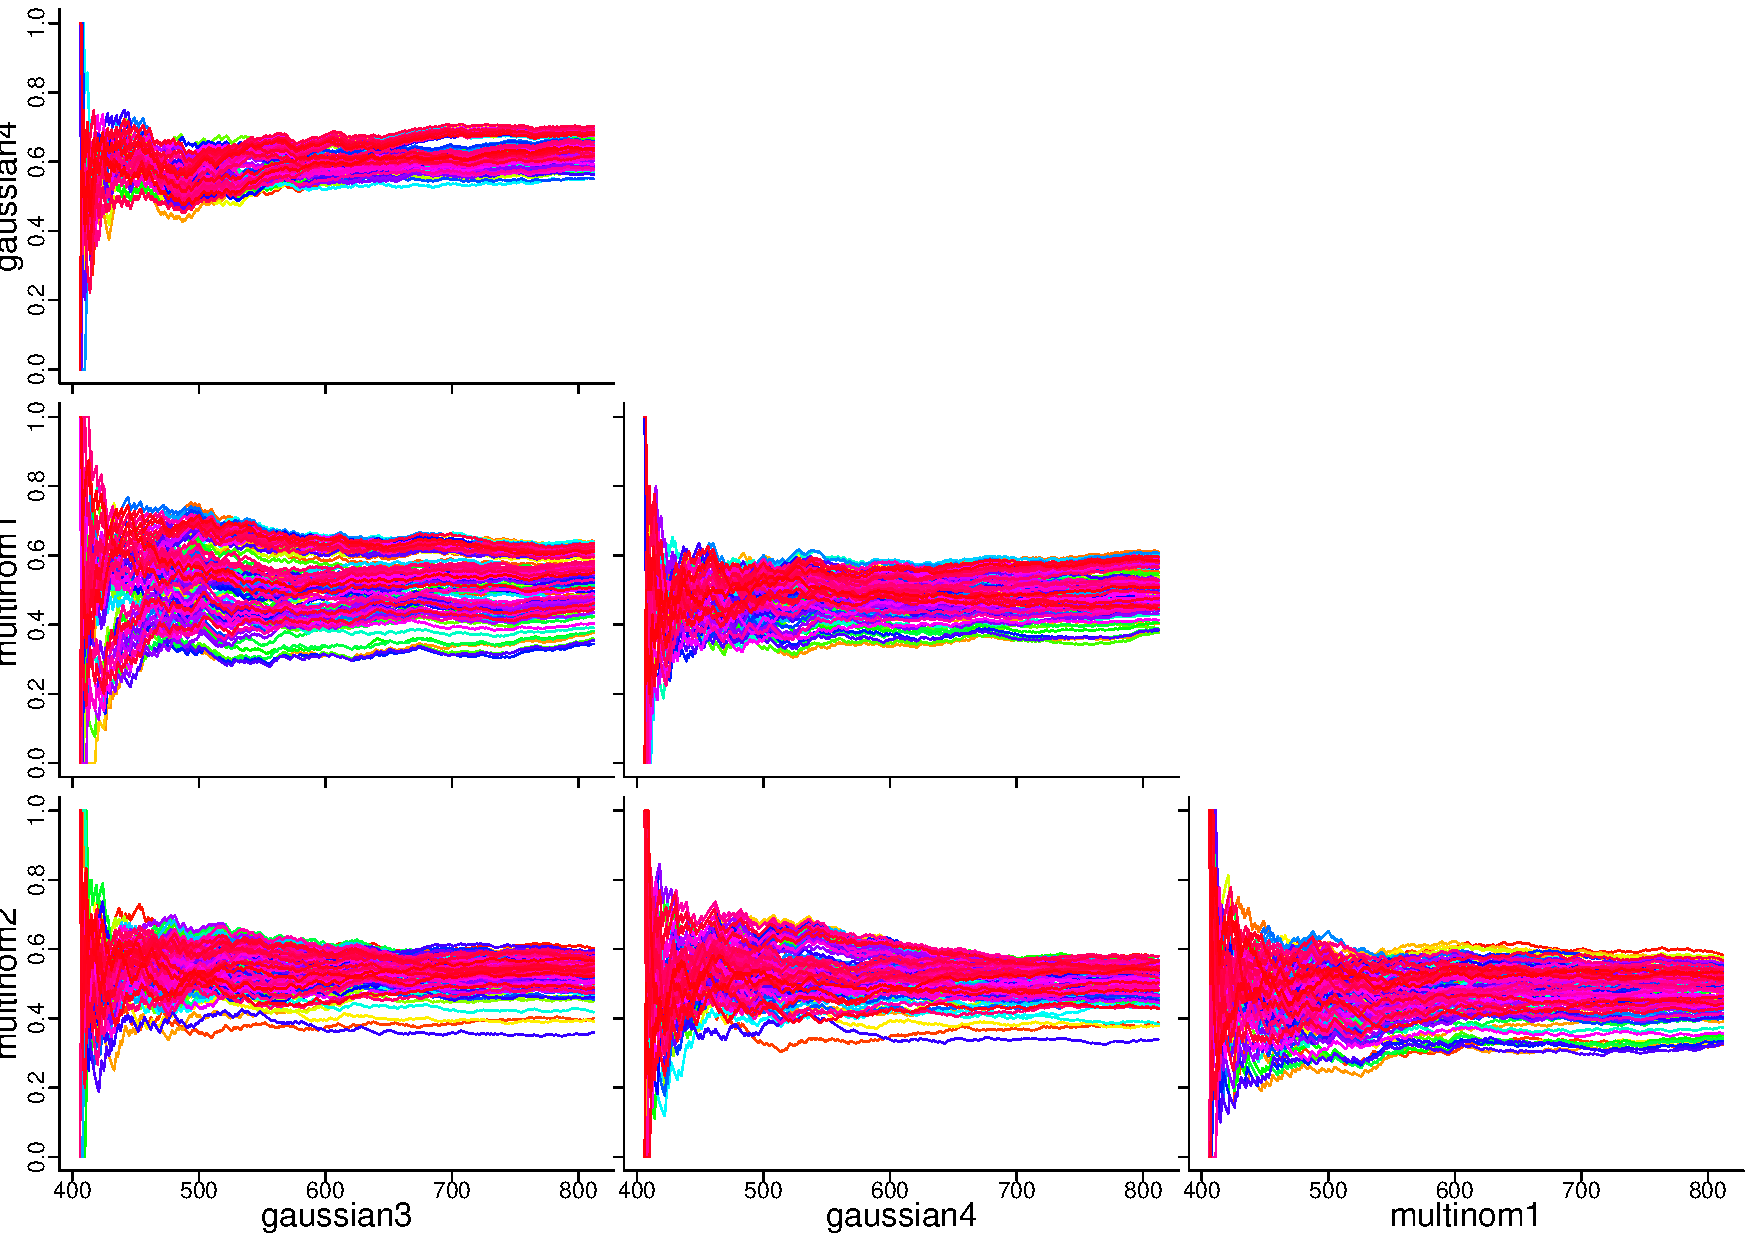
\includegraphics[width = 0.95\linewidth]{Plots/agreement.pdf}
\caption{Allocation agreement for MDI run using 4 datasets}
\end{figure}
\newpage
\begin{figure}[htbp]
\label{fig:agreement_hist}
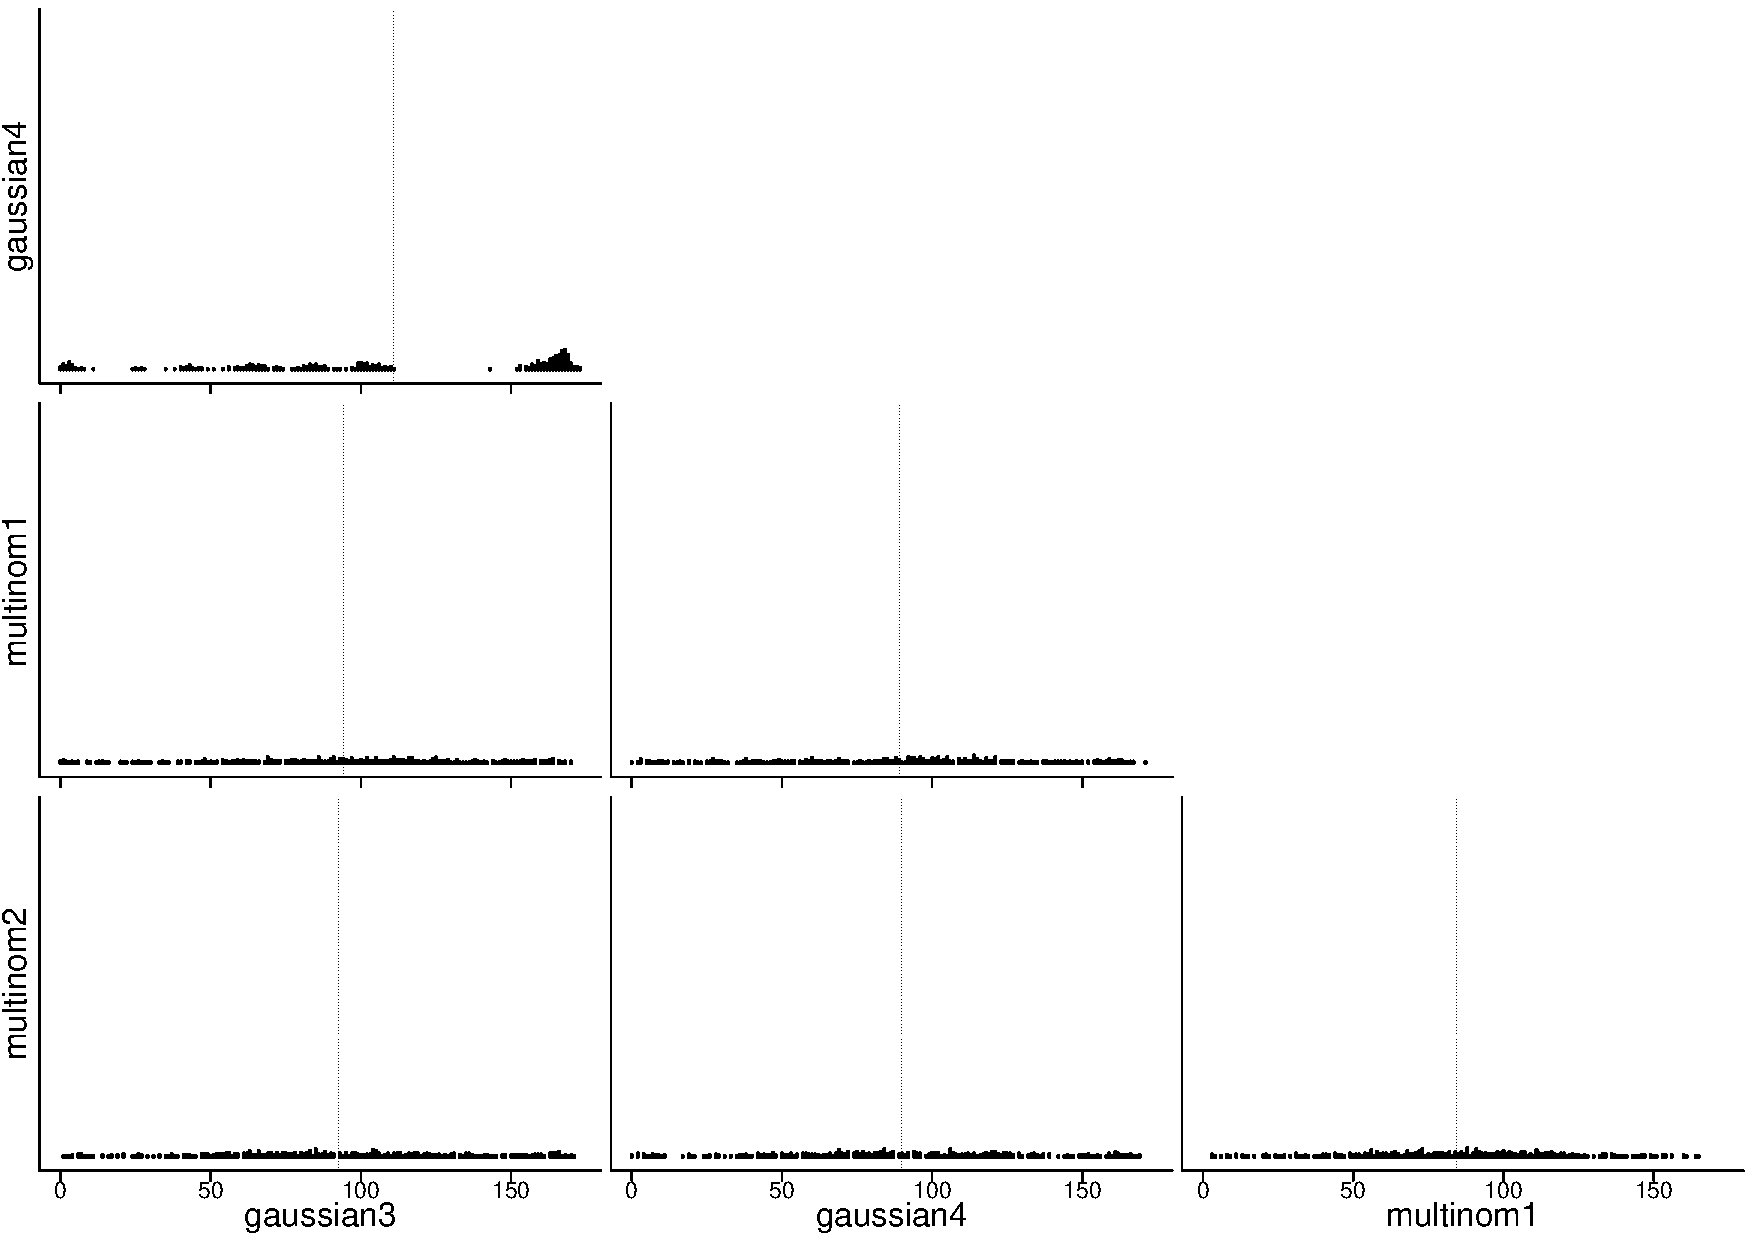
\includegraphics[width = 0.95\linewidth]{Plots/agreement_hist.pdf}
\caption{Allocation agreement histogram for MDI run using 4 datasets}
\end{figure}
\end{landscape}

\end{document}